\begin{frame}[label=current]
\frametitle{Scalar Triple Product}
\begin{columns}
\column{0.25\textwidth}
  \psfrag{u}{$\textbf{u}$}
  \psfrag{v}{$\textbf{v}$}
  \psfrag{w}{$\textbf{w}$}
  \psfrag{uxv}{$\textbf{u}\times \textbf{v}$}
  \psfrag{ow}{$\textbf{r}$}
  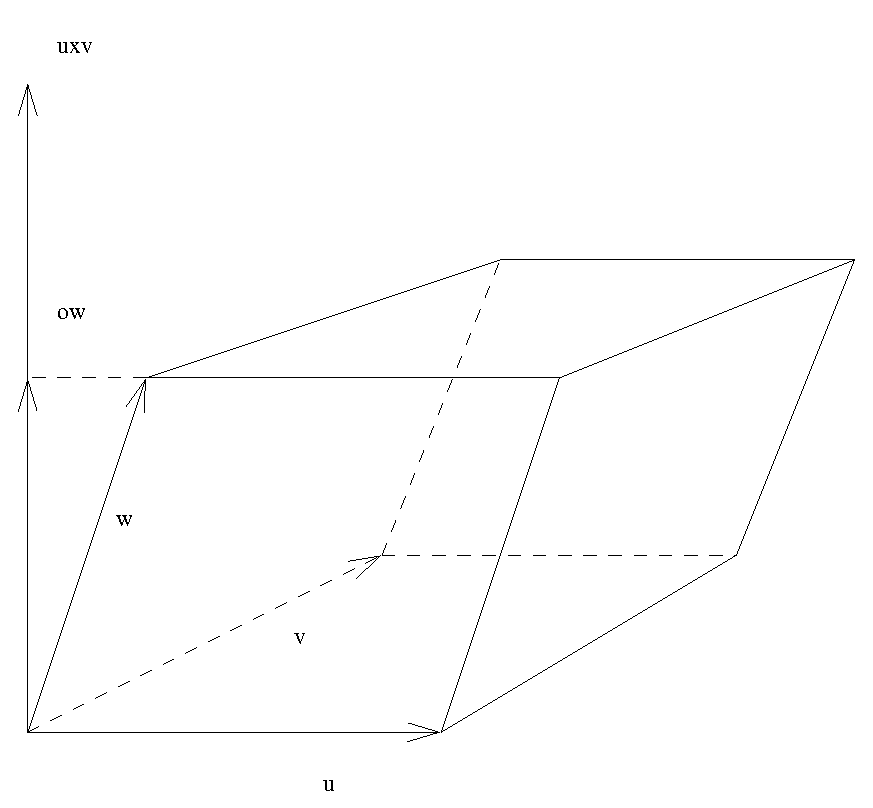
\includegraphics[height=1in]{../../modules/vectors/pictures/ok-volume_box.eps}

\column{0.75\textwidth}
\begin{itemize}
\item $A$, $B$, $C$, $D$ points in space;
\item<2-> $\textbf{u} = \textbf{AB}$, $\textbf{v}=\textbf{AC}$, $\textbf{w}=\textbf{AD}$;
\item<3-> $R=R(\textbf{u},\textbf{v},\textbf{w})$: box on sides $\textbf{u}$, $\textbf{v}$, $\textbf{w}$.\pause
\item<4-> $\text{Vol}(R) = |\textbf{u} \times \textbf{v}| |\textbf{r}| = |\textbf{u} \times \textbf{v}| \, |\textbf{proj}_{\bm{u} \times \bm{v}} \textbf{w}| =
|\textbf{w} \cdot (\textbf{u} \times \textbf{v})|\; .$
\end{itemize}
\end{columns}
\uncover<5->{
\begin{definition}
The quantity $\textbf{w} \cdot (\textbf{u} \times \textbf{v})$ is called the scalar triple product of $\fcv w, \fcv u, \fcv v$.
\end{definition}
}
\uncover<6->{
\begin{itemize}
\item If $\textbf{u} =\langle u_1,u_2,u_3\rangle$,
$\textbf{v} =\langle v_1,v_2,v_3\rangle$, and $\textbf{w} =\langle w_1,w_2,w_3\rangle$, then
%
$$\textbf{w} \cdot (\textbf{u} \times \textbf{v}) = \left|
\begin{array}{ccc}
w_1 & w_2 & w_3 \\
u_1 & u_2 & u_3 \\
v_1 & v_2 & v_3
\end{array}
 \right|$$
\end{itemize}
}
\end{frame}